\begin{longtable} { | c | p{12cm} | c | } 
\hline
	ID 	&	Issues	&		 Es. hours \\\hline
	12 	&	Add sequence button placement is not intuitive	&	16 hours \\\hline
\caption{Issue ID 12}
\label{tab:spr3_addsequencenotintuitive}
\end{longtable}

When the costumers was editing a sequence, they found it un-intuitive that you had to press the large `framed plus' at the end of the sequence as shown in figure \ref{fig:Old_editSequence}. Furthermore when you had a long sequence (above 4 pictograms), you would have to scroll in order to find the `plus button'. We decided to add an alternative to the already existing method, and added a simple button. This way the clients have multiple ways to edit the sequences, and could use whichever they see fit \note{Tilføj billede af den nye add sequence button}.

\begin{figure} [h!]
\centering
\begin{minipage}{.7\textwidth}
\centering
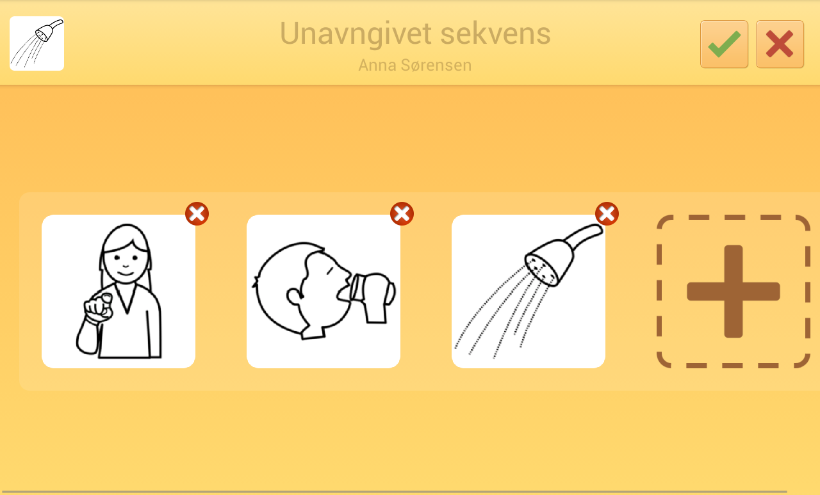
\includegraphics{Pics/Sprint3/EditModeCropped}
\caption{A picture of the editable name before}
\label{fig:Old_editSequence}
\end{minipage}\hfill
\end{figure}